%--------------------------------------------------------
\begin{frame}
\frametitle{Nuclear Suppression}

\begin{columns}[T,onlytextwidth]

%--------------------------------------------------------
% Left
%--------------------------------------------------------

\column{0.52\textwidth}

\centering
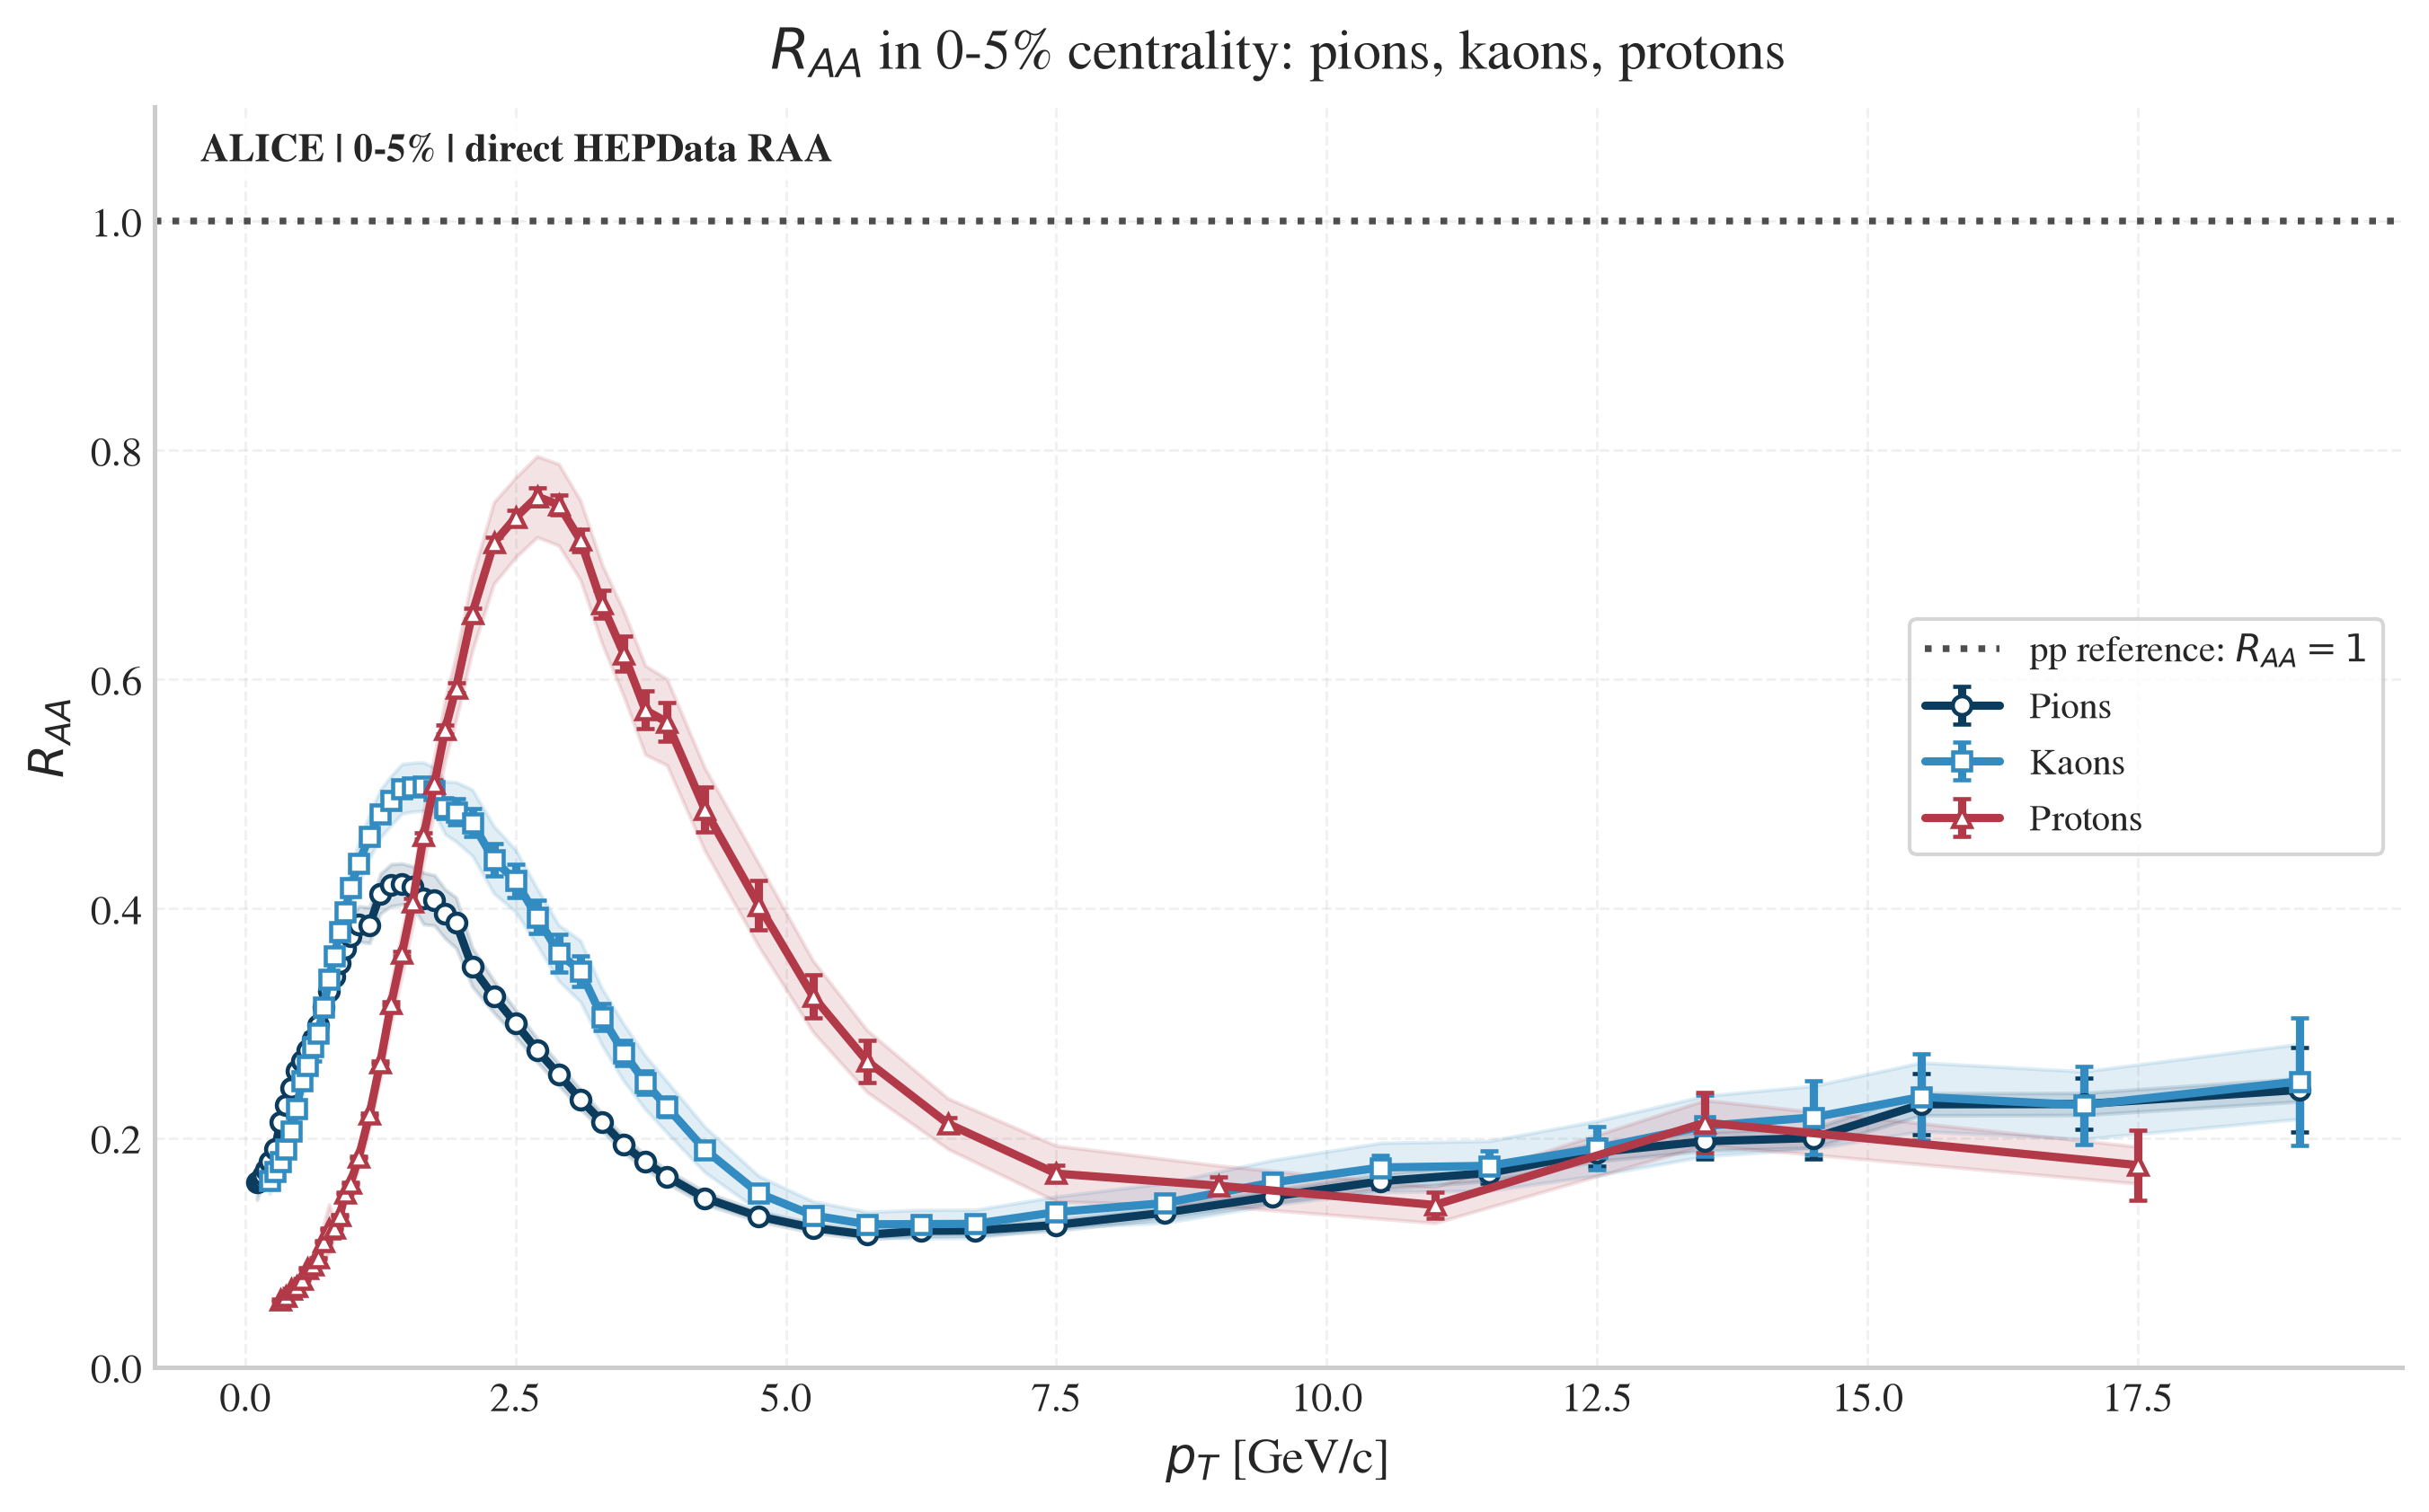
\includegraphics[width=\linewidth]{img/qgp-nuclear-supression.png}

\begin{block}{Jet quenching}
\small
Hard-scattered partons lose energy while traversing the QGP through
multiple interactions with the medium. As a consequence, fewer
high-$p_T$ hadrons are reconstructed, leading to
$R_{AA}<1$.
\end{block}

{\tiny Data source: HEPData 10.17182/HEPData-ins1759506-v1.}

%--------------------------------------------------------
% Right
%--------------------------------------------------------

\column{0.44\textwidth}

\small

\textbf{Nuclear modification factor}

\vspace{-0.15cm}

\[
R_{AA}(p_T)=
\frac{1}{\langle N_{\rm coll}\rangle}
\frac{dN_{AA}/dp_T}
{dN_{pp}/dp_T}
\]

\vspace{0.6cm}


\begin{itemize}
\item $R_{AA}=1$: binary collision scaling.

\item $R_{AA}<1$: suppression due to medium-induced energy loss.

\item Intermediate $p_T$: protons are less suppressed than mesons.

\item High $p_T$: all hadron species exhibit a similar suppression.
\end{itemize}

\end{columns}

\end{frame}